\chapter{Problem definition}
\section{Foreword}
One edge of Medialogy is systems built to react accordingly to humans. This system is called Visual Computing. There are several not least good topics that apply to this kind of technology. One area in which image processing and specific object recognition is used, is surveillance. By implementing some custom made software, one will be able to monitor a specific target group or process. In addition to the semester project two mandatory courses on the third semester of Medialogy are of interest to our semester project.\\
The first course is called Image Processing and it is primarily based on understanding the theory of a picture and tools to manipulate the pixel values within. Knowledge such as the principle of 8-bit, the RGB color system, histograms and using threshold to segment a picture are some of the tools learned from the course.\\
The second course used for the semester project is Procedural Programming, in which programming skills in C++ are learned. The theoretical background for programming is necessary to complete image manipulations, based on methods learned in Image Processing.

As for project themes eleven subjects were presented to us in which we had to make a list of three wishes in prioritised order. These eleven subjects were very unspecified projects so it is up to the group to form its personal project. \\
The eleven subjects presented was:

\begin{itemize}
\item Image Processing for Fun Utilizing an Industrial Robot
\item Image Processing for Ambient Intelligent Robots
\item Interactive Floor
\item Interactive Book
\item Interactive Drawing Game
\item Interactive Arcade Game
\item Emergency system for old people that have fallen
\item Thermal Sock Puppet Show
\item Body Motion Controlled Exercise Game
\item Mobile app for recognizing electric components
\item Hj{\o}rring Library
\end{itemize}

After reading into the different project proposals the group decided which three subject to apply for in prioritised order:

\begin{enumerate} 
\item Hj{\o}rring Library 
\item Interactive Floor 
\item Image Processing for Ambient Intelligent Robots 
\end{enumerate}

\section{Establishing collaboration with Hj{\o}rring Library}

To great delight our group were chosen to work with Hj{\o}rring Library which was our first priority. A meeting was arranged and the group together with other groups from third and fifth semester of Medialogy travelled to Hj{\o}rring to meet the library staff. In addition the groups were let loose in the library to check locations for potential projects.\\
After talking to some of the staff, more specific our contact person Martin J{\o}rgensen, some general ideas emerged, so it was decided to go back to the group room at NOVI to do some brainstorming within the group.

The first idea that emerged, included scanning of barcodes on books in the library. The idea was that the shade of people trespassing on the walkway where the canvas was placed, would be projected onto the canvas. The conceptual idea was that people would explore the library and depending on the book gathered and scanned, some specific graphic would appear on the canvas. An example could be scanning a fairy tale written by H.C. Andersen which would then produce a hat on-top of the user.

After conferencing with the supervisor, Thomas Moeslund, and the co-supervisor, Andreas M{\o}gelmose, it was decided that the conceptual idea needed to be narrowed down to a more specific subject field. The second idea emerged that we should focus mainly on fairy tales and first of all work around H.C. Andersen, which meant adding a top hat on-top of the users.

An email was sent to Martin J{\o}rgensen concerning the concept for the third semester project and also the location of the project. Martin liked the idea, but had some concerns to identify the period in which the project would fit the library. Hj{\o}rring Library work around specific topics that change every 8-12 weeks. One of the upcoming themes of interest at the library was Christmas which runs from the 2nd week of November until the last week of December. Another idea then emerged in the group towards creating a project for December. Instead of working with the H.C. Andersen theme, it was decided to work with father Christmas and to add a Christmas hat on-top of trespassing users of the library. Martin was fond of this idea and so a new meeting was arranged in order to settle on a suitable location at the library for our project.\\
Two members of the group travelled to Hj{\o}rring Library to participate in the meeting with Martin. The outcome was a more specific plan on the project concerning the:

\begin{itemize}
\item The position of the project
\item The equipment that was desired to borrow
\item The light conditions
\end{itemize}

The position of the project will be on the walkway from the reception desk to the core of the library, which Martin believed would be an ideal position for the project, as the light conditions are controllable. In addition to that he knew from experience that people tend to use that walkway either to enter or exit the library, as it is the shortest route.

\begin{figure}[htbp]
\centering
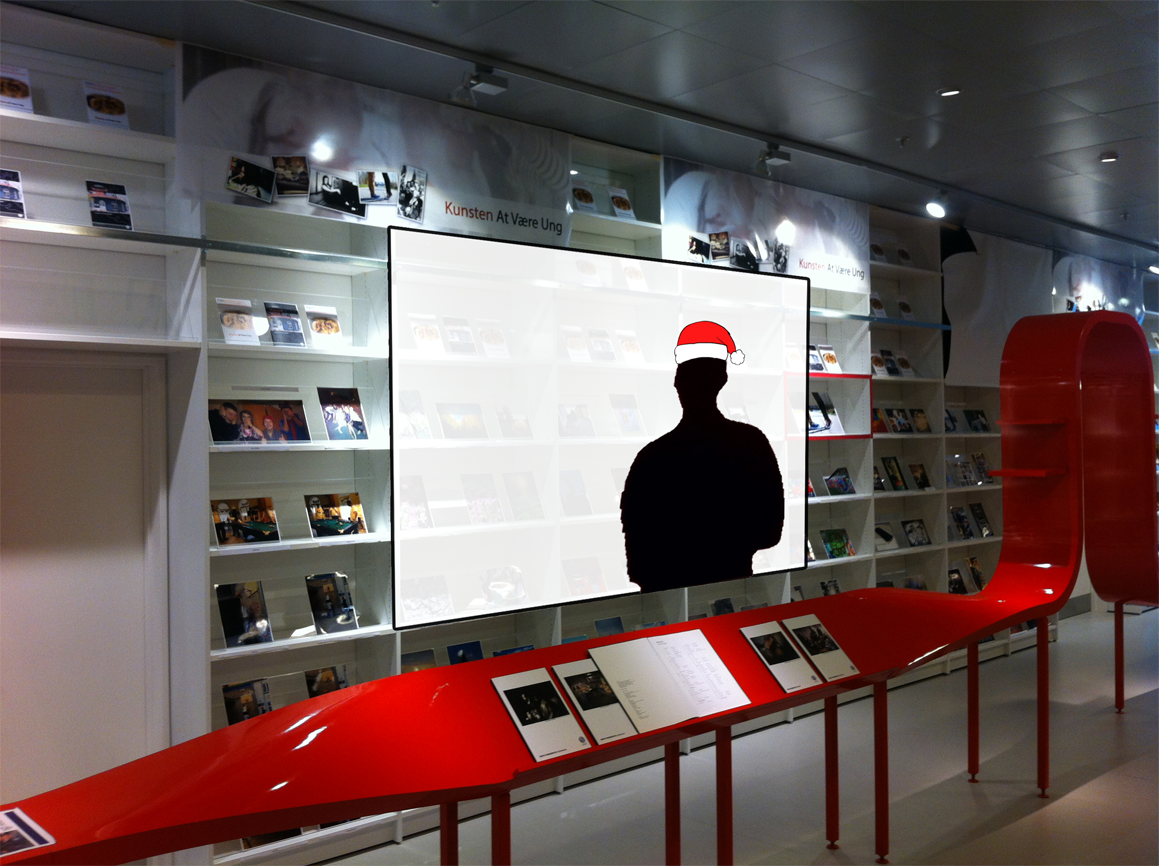
\includegraphics[width=1.00\textwidth]{Pictures/HjoerringLibrary/LocationJohannesHat.jpg}
\caption{Location a Hjørring Library}
\label{fig:concept_art}
\end{figure}
Figure \ref{fig:concept_art} illustrates the setup at the library. A canvas with the proportions 3 * 2.25 meters will be positioned directly on the bookshelves seen in the background of the picture.

\subsection{The initial goal}
One thing that Martin was interested in, was knowing the ambitions for the project and what to expect. There had been a talk within the group about ambitions for the project at Hj{\o}rring Library. Considering the knowledge in programming and image processing, being ready to present the prototype the 1st of December was a part of the initial goal. Previously Martin told us that the Christmas theme would run from the second week in November, until the last week in December, therefore a 3 week run-time period was a desirable goal.\\
As for the initial goal, Martin expressed his excitement by letting us know that it was very ambitious, but that we should not be intimidated and that he hoped we would succeed. Furthermore he let us know that he would like to contact the designer in charge of the exhibitions at the library to create some interesting scenery for the project. Lastly he expressed that in case we would not succeed to finish the prototype for 1st of December and run for three weeks period, he would like to know, so that he could contact the designer and tell her to do some backup exhibition.

\section{Technical point of view}
The basic idea is to have a canvas on which the shade of the person is projected together with the Christmas hat added to the top of the head. For that some tools are needed:

\begin{itemize}
\item A web camera to gather input about people trespassing
\item A laptop to run the program code
\item A projector to display the output from the computer
\item A canvas on which the output is projected on
\item Controllable lights/light conditions
\item Power, cables etc.
\end{itemize}

Together with a projector capable of projecting a relative huge output 3*2.25 meters, the laptop running the program code will also be connected to a web cam. A canvas in above-mentioned size will have to be made and placed on-top of the book-shelves illustrated on figure 1.1.

\subsection{Ground zero}
The first step into developing some usable software, was to write some scrappy code that would run and produce a measurable output. This was done by dividing the entire group consisting of 6 people into 2 smaller groups of 3 people, to come up with a solution on how to produce a segmentation of the video input. A competition within the group turned up to create the best program code in 3 days to be presented. And so the "winner's" code or parts from both projects would be incorporated in a testable file.\\
At the end of the week, two programs were ready to be tested. Both programs were able to do same things, only the code differed. Some of the techniques used were: Median filtering, morphology(opening/closing), background subtraction, conversion from a colored image to a gray-scale image and most important a first draft of the BLOB analysis, needed to analyze the shape of the head where the Christmas hat is to be placed.\\
One team did however create some custom made structures so that all would be able to include their own functions in the program without interfering with others. Therefore it was decided to use that program to implement the different functions.

\subsection{Running the first test}
As the first prototype of the program was completed, it was decided to test the piece of code written and also the equipment given. Mainly because it was of great importance to check the outcome of the input video, considering the fps(frames per second) and the static threshold set. 

\begin{figure}[htbp]
\centering
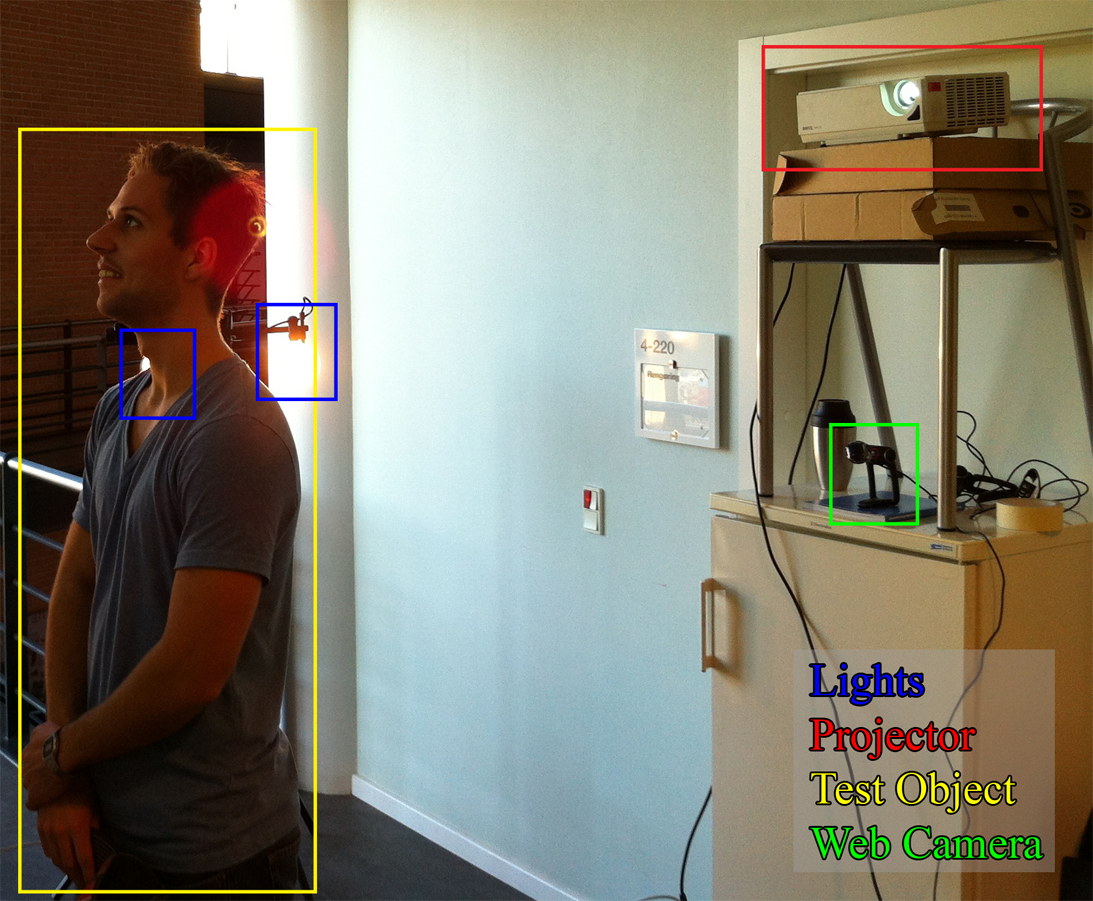
\includegraphics[width=1.00\textwidth]{Pictures/Test/TestSetup.jpg}
\caption{Picture from Testing the Infrared Camera}
\label{fig:Picture from Testing the Infrared Camera}
\end{figure} 

Figure \ref{fig:Picture from Testing the Infrared Camera}  illustrates the initial setup for the first prototype testing. \\
At first the ordinary web camera was used, but due to change in light conditions from the objects trespassing, which caused glittering on the output, it was decided to use the infrared camera. In addition to the infrared camera, four light bulbs were used to \fixme{feed (find synonym)} feed the infrared camera with information regarding the test person. This produced a somewhat good output of the testperson, though one problem still remained. Once the testperson turned 90degrees\fixme{degrees (math symbol)}. the head became much smaller and didn't look very precise on the output, in addition the Christmas hat would also be misplaced.\\
The solution to this turned out to be illuminating the background instead of the person, which produced a really great output, seen on figure \ref{fig:max_subtracted}.


\begin{figure}[htbp]
\centering
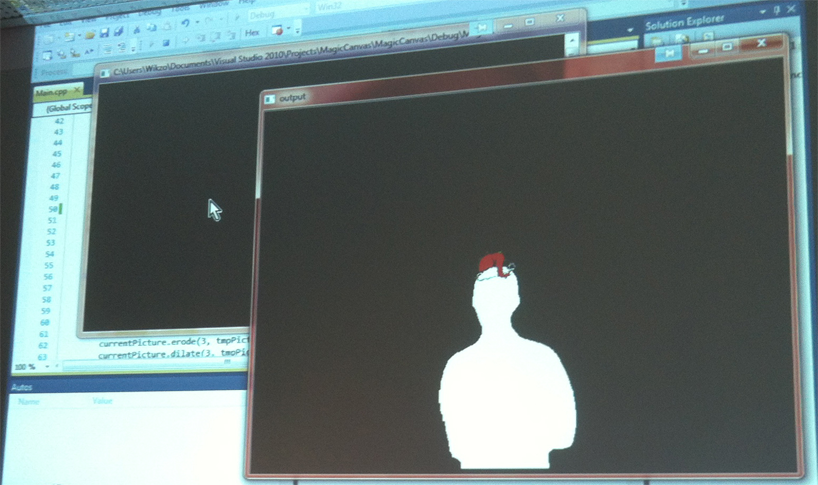
\includegraphics[width=1.00\textwidth]{Pictures/Test/MaxSubtracted.jpg}
\caption{Complete subtraction of object outputted as binary picture.}
\label{fig:max_subtracted}
\end{figure}


\section{Supervisor meeting with Andreas 14th of November}
The 14th of November a supervisor meeting was arranged with the co-supervisor Andreas M{\o}gelmose. The meeting was initiated to receive some valuable feedback on the prototype testing and secondly some concerns regarding the programming had arisen. Currently the program ran with 2-3 fps, due to the mathematical calculations performed in the program, such as looping through the entire image's pixel values several times.\\
To this several not least good suggestions were given, such as adjusting the BLOB analysis to a more specified point of interest and also to include another method of subtracting the background called \textbf{ViBe}.

\subsection{Using an avatar instead of shape}
 \begin{itemize}
\item Reduce the image processing to the region of interest, perhaps discarding 60-70percent\fixme{percent(math symbol)}.
\item Producing a nice real-time output in form of pixies with hats.
\item Pixies can be a recorded scene that will be looped.
\item Describe the use of multiple threads in programming.
\end{itemize}
 
\section{Initial Vision}
To summarize on the above-mentioned in regards to the equipment, the skills of the individual members of the group, the theme and the actual concept.\\
Considering the hypothesis that all time in the world was given along with all money needed, the outcome of this project would without doubt be mind blowing\fixme{mind blowing(find synonym)}. Limited by time, skills and equipment an alternative plan was to be worked out and adapted to what was possible. Producing an output of the entire image, performing several mathematical operations are simply too heavy work for the program in extend to the programming skills of the group. The skills at programming are simply not advanced enough at doing optimized algorithms, to make the program run smooth in real time. \\
Therefore research towards analysing regions of interest on an input was performed. This would make it possible to discard up to 60 percent of the mathematical operations needed\fixme{percent(math symbol)}, which ultimately should produce more frames per second, when running the program. In addition this should enhance the user experience as the tracking of the Christmas hat would be much smoother.
\\
Some of the goals, which are of interest to this project is that people can engage in the game at two levels. Given that people can engage passively in the game, simply by trespassing the area of the project without minding the canvas, on which the Christmas hats will be navigated around. Secondly it's of interest that people can engage actively in the game by moving side to side and back and forward to create an illusion of being there. In continuity of that, participants might tell their acquaintances/friends about the game and bring them along.
\\
Based on reaching the above-mentioned goals by engaging people on two levels at the library, the initial vision of this semester project is the following. "How do we succeed in engaging visitors at Hjørring Library to use our product on two levels, both passively and actively."






